\section{Detailed control design for agreed plant section}
\label{sec:subsec}

\subsection{Control objectives}

\subsection{Key control loops}

\subsubsection{Reactor R201 temperature control}
\begin{figure}[H]
    \centering
    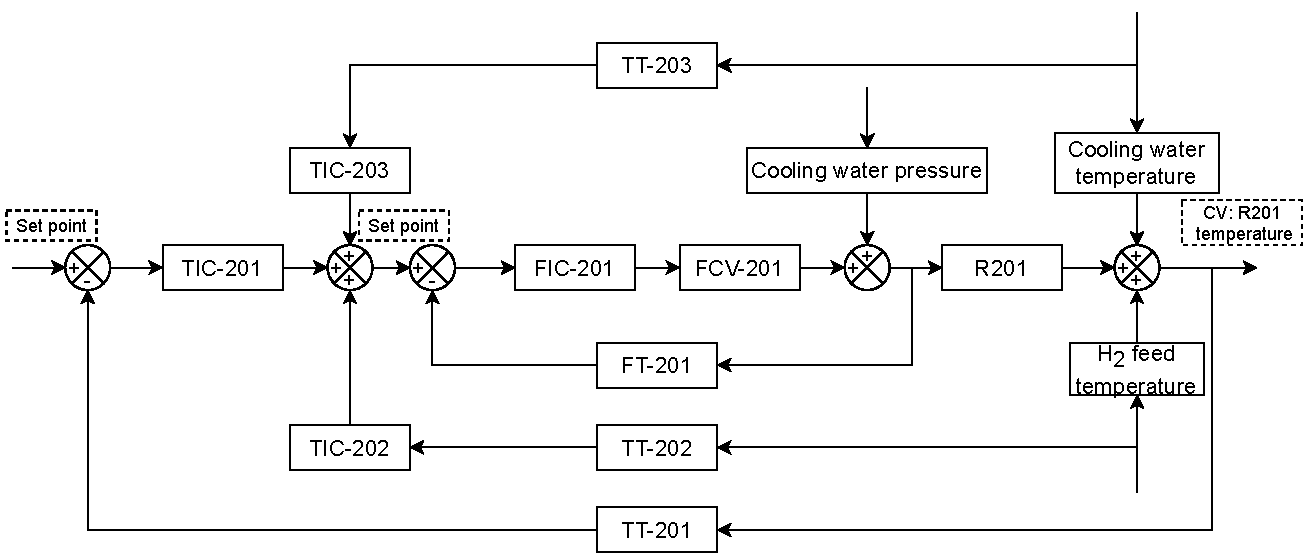
\includegraphics[width=\linewidth]{chapters/4-operation-control/4-Figures/R201-TC.pdf}
    \caption{}
    \label{fig:R201-TC}
\end{figure}

\subsubsection{Reactor R201 pressure control}
\begin{figure}[H]
    \centering
    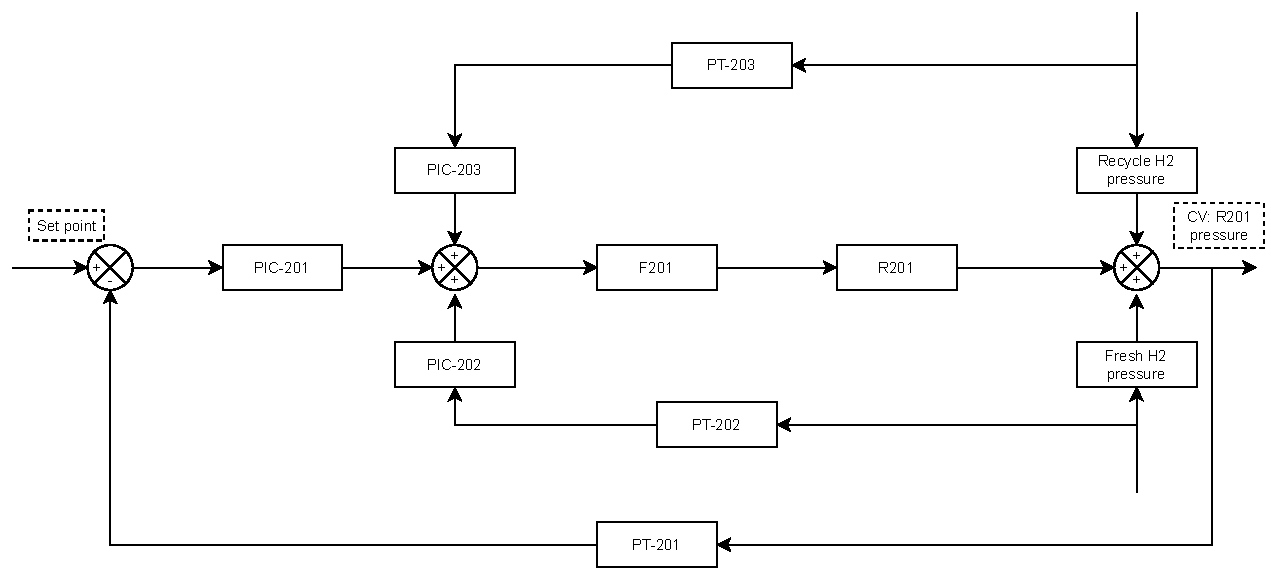
\includegraphics[width=\linewidth]{chapters/4-operation-control/4-Figures/R201-PC.pdf}
    \caption{}
    \label{fig:R201-PC}
\end{figure}

\subsubsection{Reactor R201 level control}
%\begin{figure}[H]
 %   \centering
  %  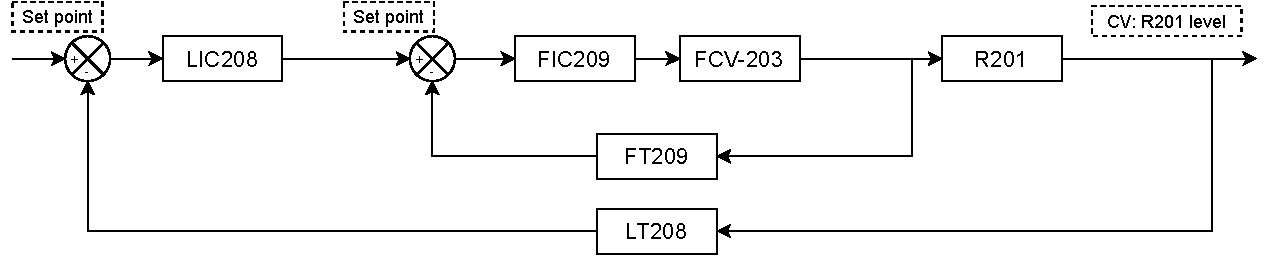
\includegraphics[width=\linewidth]{chapters/4-operation-control/4-Figures/R201-LC.pdf}
   % \caption{}
    %\label{fig:R201-LC}
%\end{figure}

\subsubsection{Reactor feed temperature control}

\subsubsection{Hydrogen recycle control}
\begin{figure}[H]
    \centering
    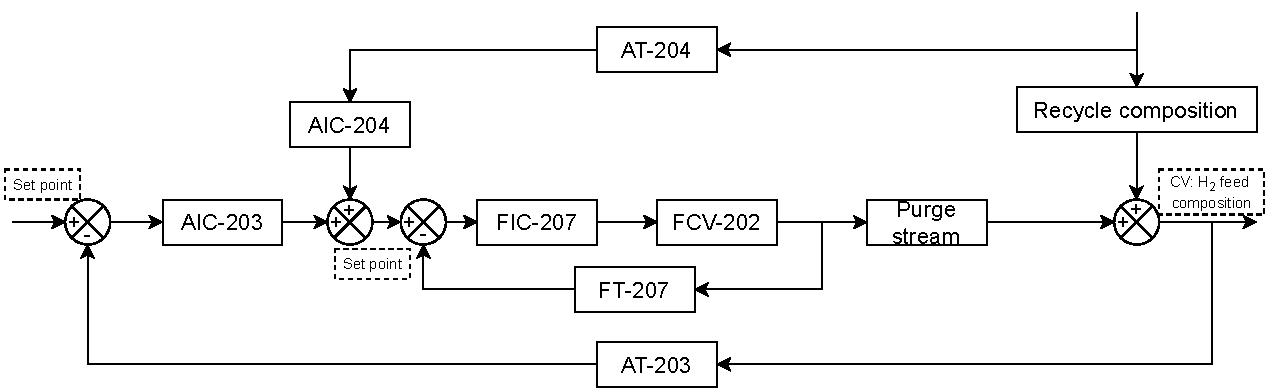
\includegraphics[width=\linewidth]{chapters/4-operation-control/4-Figures/V202-CC.pdf}
    \caption{}
    \label{fig:V202-CC}
\end{figure}

\subsubsection{Reactor outlet flow control}
\begin{figure}[H]
    \centering
    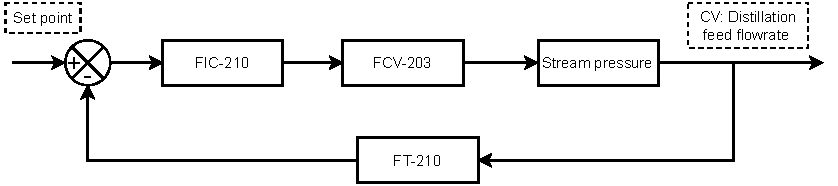
\includegraphics[width=\linewidth]{chapters/4-operation-control/4-Figures/V201-FC.pdf}
    \caption{}
    \label{fig:V201-FC}
\end{figure}


\subsubsection{Control of pressure reduction valve V201}
\begin{figure}[H]
    \centering
    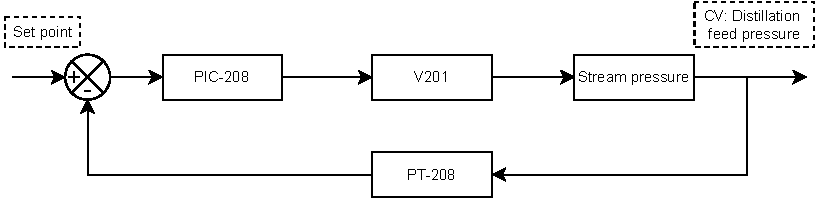
\includegraphics[width=\linewidth]{chapters/4-operation-control/4-Figures/V201-PC.pdf}
    \caption{}
    \label{fig:V201-PC}
\end{figure}

\subsubsection{Distillation column S201 pressure control}
Pressure in distillation columns is regarded as one of the most important parameters to control well, as it not only affects the relative volatilities of the heavy and light keys, but also the shape of the vapour-liquid phase equilibrium curves which determine the compositions of the top and bottoms products of the distillation column. There are several options for for pressure control, such as controlling the vapour flow that is vented from the reflux drum, condenser duty, reboiler duty, recirculation of cooling fluid in the condenser or addition of inerts. Hence the choice of manipulated variable needs to be made carefully considering the relative direct impacts and time delays of each manipulated variable. Controlling the vapour flow that is vented from the reflux drum is the simplest control to implement and usually provides the fastest response as the amount of gas holdup in the column directly affects its pressure. In addition, the amount of vapours in the reflux drum S204 is much larger compared to the condensed liquid flow, so the direct impact of vapour flowrate on column pressure would be large. This avoids a situation where the flow control valve becomes saturated and unable to regulate pressure effectively. 

An optimal feedback control was designed with the vapour flowrate from the reflux drum as the manipulated variable. A pressure transmitter (PT-206) measures the pressure in the column, which is monitored by a pressure controller (PIC-206) that regulates a flow control valve (FCV-205) on the vent stream from the reflux (Figure \ref{fig:S203-PC}.

\begin{figure}[H]
    \centering
    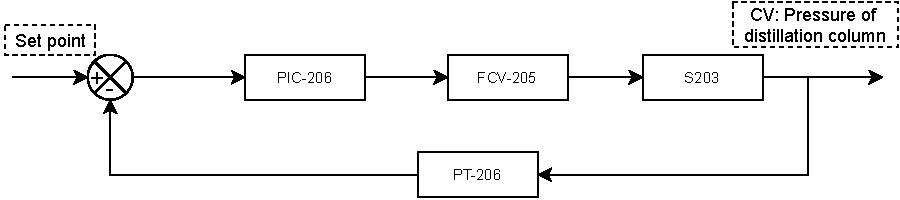
\includegraphics[width=\linewidth]{chapters/4-operation-control/4-Figures/S203-PC.pdf}
    \caption{}
    \label{fig:S203-PC}
\end{figure}

\subsubsection{Bottom stream composition control}
A composition control loop in the distillation column is also necessary to ensure a high recovery of o-toluidine. Since o-toluidine is found in the bottoms stream, reboiler duty was chosen as the manipulated variable in order to reduce the lag time of the controller. A composition analyser (AT-205) measures the concentration of o-toluidine in the bottoms stream and a composition controller (AIC-205) controls the reboiler duty by manipulating a flow control valve (FCV-207) on the saturated steam. 

A composition analyser was chosen to allow direct online measurements of the o-toluidine concentration, providing primary data to plant operators regarding this important performance indicator. However, composition analysers often have a slow dynamic response, leading to long measurement lags that result in a delay in the response of the control system. This sluggish behaviour would lead to the concentration of the bottoms fluctuating. To mitigate this, the temperature of the column is used as an inferential sensor to control the product composition, and is assigned as a slave controller under the master composition controller. Temperature sensors have quicker dynamic responses and can be correlated well to product composition. Controlling the temperature of the column is also crucial to a safe operation of the plant. Figure \ref{fig:S203-CC} shows the temperature controller (TIC-207) that receives its setpoint from the master composition controller (AIC-205), and outputs a signal to the flow control valve FCV-207.

\begin{figure}[H]
    \centering
    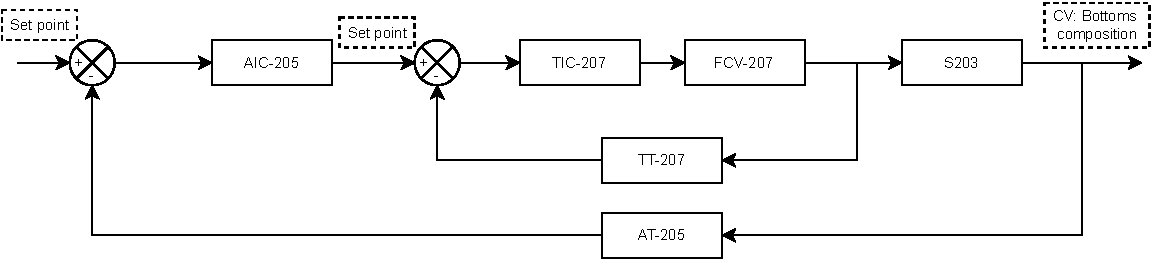
\includegraphics[width=\linewidth]{chapters/4-operation-control/4-Figures/S203-CC.pdf}
    \caption{}
    \label{fig:S203-CC}
\end{figure}

\subsubsection{Distillation column S201 level control}
The liquid level at the bottom of the distillation column S201 is an important inventory to control to to prevent the reboiler from drying up and weeping to occur in the column. Since the reboiler duty is already being used in composition control, the most direct way of controlling the level is the bottoms flowrate out of the reboiler. Since the column and reboiler are connected, draining more liquid from the reboiler would draw more liquid from the column and vice versa. Due to the reboiler being able to store a certain amount of liquid inventory, a lag between the response of the actuator and the level is expected. While in most cases a simple feedback controller is sufficient (see Figure \ref{fig:S203-LC}, experimental data would confirm if more advanced systems are needed to compensate for a large time delay. 

\begin{figure}[H]
    \centering
    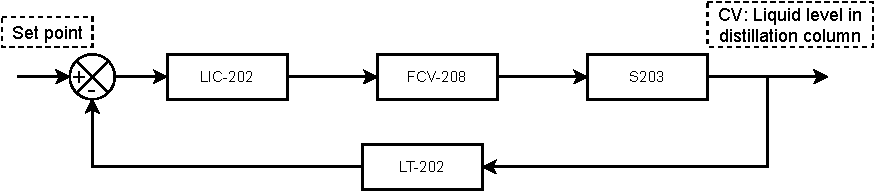
\includegraphics[width=\linewidth]{chapters/4-operation-control/4-Figures/S203-LC.pdf}
    \caption{}
    \label{fig:S203-LC}
\end{figure}

\subsubsection{Reflux drum S204 level control}
Similar to the level control in the column, controlling the level of liquid in the reflux drum is required for stable operation of the column. Letting the drum run dry would lead to no reflux returning to the column, which would affect the separation efficiency of the light and heavy components. The manipulated variable for the liquid level was chosen to be the tops product flowrate, as it was desirable to maintain a constant reflux ratio to the column in order that the energy required to achieve the desired degree of separation would remain constant. A level transmitter (LT-203) sends a signal to the level controller (LIC-203) which controls a flow control valve (FCV-206) on the tops outlet stream, as shown on the P&ID. 

\subsubsection{Heat duty of condenser H203 control}
The condenser in a distillation column provides cooling to condense the vapour exiting from the top of the column. It is usually desirable to operate the condenser at maximum duty, as reflux to the column has to be in a liquid state. Thus it is important to ensure that any disturbances to the cooling water flowrate and temperature are mitigated with a control loop. A cascade control was proposed as the best way to account for disturbances in these two parameters, with the slower temperature loop as the master control and flowrate as the slave.


\begin{figure}[H]
    \centering
    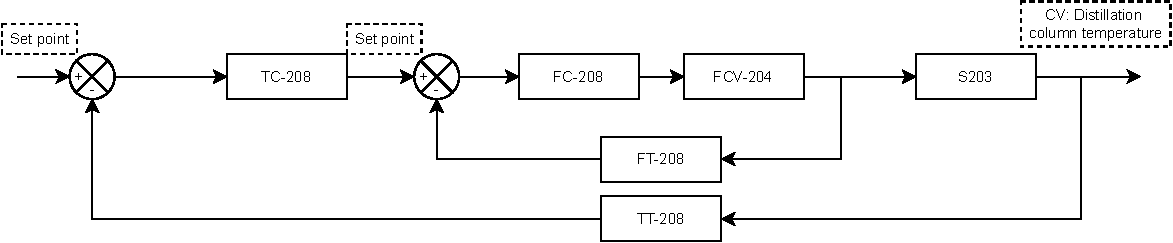
\includegraphics[width=\linewidth]{chapters/4-operation-control/4-Figures/S203C-TC.pdf}
    \caption{}
    \label{fig:S203C-TC}
\end{figure}


\subsubsection{}

\subsection{Safety design}

\subsubsection{Alarms and emergency trips strategy}

\subsubsection{Alarms and safety interlocks design}